\documentclass[lang=cn,cite=super]{elegantpaper}
\usepackage{bm,appendix,graphicx}
\title{低成本普惠型智能家居方言指令转换器的研究}
\author{陶理}
\date{}

\begin{document}
\maketitle
\begin{abstract}
\end{abstract}
\newpage
\begin{center}
    \tableofcontents
\end{center}
\newpage
\setcounter{section}{-1}
\section{引言}
随着普通话的推广,为了更好地与各族人民交流,方言的盛行注定会成为过去时。不过,各地迥异的方言是中华民族传承千年的瑰宝。以吴语为例:现如今普通话已经只剩下四个声调,即所谓的阴平、阳平、上声、去声,但是在古汉语中还有一个声调为入声,在古诗文的韵律中时常出现;如在浙江义乌话中,声调达到了10个。因为有入声,所以使用方言阅读古诗文能够接近古人在创作时的读音,相较于普通话更有韵味。全中国共有约10种方言大类,如图\ref{fig:chinese-lanaguages-map}所示,其中包括吴语、粤语等.而各地区又有不同的发音、措辞上也有区别,如在浙江,由于丘陵地势,不同地域的交流不频繁,使得同属吴语系的发音天差地别。
\begin{figure}[h]
    \caption{\label{fig:chinese-lanaguages-map}主要方言分布地图}
    \centering
    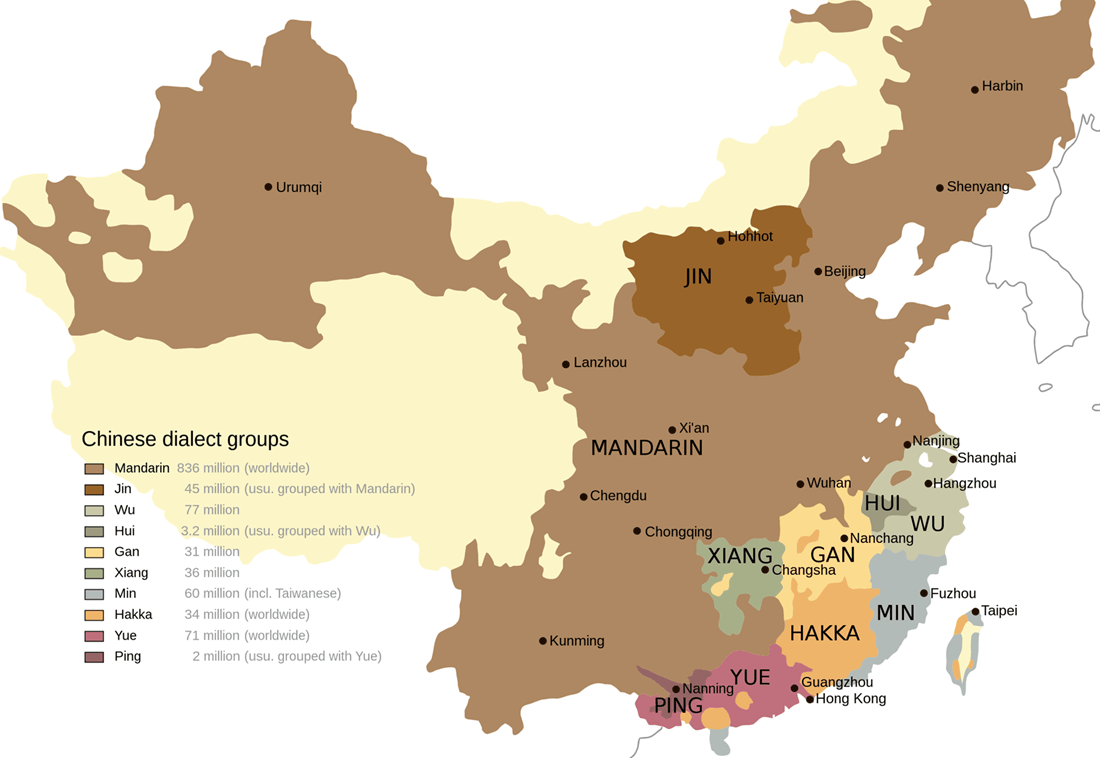
\includegraphics[scale=0.34]{chinese-lanaguages-map.png}
\end{figure}

方言的多样性也同样是方言在文化上重要性的体现。但是如今的方言正在高速消亡,多样性在飞速下降,特别是小众方言。沪剧、川剧、粤语歌曲等流行的艺术形式使得大方言得到了一定程度上的新生,而且如今讯飞科技等公司、组织也研发了此类大方言转换为人工智能的算法,并已经付诸实践。而小众方言在使用人群数量上无法与大方言相比,自然在被关注度上也无法与大方言争锋。但是在这些小众方言流行的地域上,新一代的年轻人同样大多都说普通话,若是没有进一步的保护措施,这类的小众方言将很快走下历史的舞台。早在2005年的11月,时任教育部语言文字信息管理司司长李宇明在接受《语言文字周报》采访时,他指出:“建立和谐的语言生活,首先要对语言多样性有充分的认识,要尊重各民族的方言,要尊重各种方言,包括尊重繁体字等历史上的文字,因为这些都是中华民族的宝贵财富。”

因此,虽然方言的小众化是不可逆的,但是及时的研究能够更多地保留这一非物质文化遗产。因此需要尽快进行研究。
吴永焕[1]就方言的保护在必要性和紧迫性的方面进行了论证,强调了要抢记方言资料,尽可能延缓方言特征消失速度;
黄涛[2]强调了方言在文化价值上的重要性;相应的保护政策也相继出台,因而保护方言是很有必要的。

另外,在高度信息化的现代社会,语音识别正在被广泛地应用和推广。在各种设施和应用场景中,语音识别的重要性也越来越高。语音识别技术使得人们可以方便地通过语音来交流、控制和感知信息,比如在使用即时通讯软件时能够进行语音输入,通过与智能音响等的对话了解天气情况,或者通过智能家居系统来进行家电控制。由于方言的发音和说话习惯与普通话大相径庭,因此使用普通话数据训练得到的语音识别模型无法准确地预测方言语音的含义。这会导致两个后果:1. 方言的使用场景减少,而更少的应用会进一步加速方言的消亡;2. 无法通过小众方言使用各种基于语音识别的应用和设施,如使用方言调用智能家居系统。

智能家居是以语音识别为基础,智能家具通过语音模型理解人的指令进而执行指令。但是语音识别模型的缺陷在于大多模型是基于普通话进行训练的,所以导致对于方言的支持很差。而对于方言识别来说,如今只有大方言的语音识别模型,小众方言并没有对应的语音识别模型。这导致说小众方言的智能家居使用者只能使用普通话进行指令的描述。而小众方言的使用者占我国总人数的很大比重。虽然现在普通话推广范围很广,但是还是有很多人(以老年人为主)对于普通话的运用并不熟练。若一致使用普通话,会降低使用方言的频率,进而会使得方言的消失速度更快,特别对于小众方言。因此针对小众方言研究方言指令转换器是十分有必要的。

在此之前,已经有许多学者就方言识别进行了研究:
武瑞丰[3]提出了人工智能在方言建档中有很大的作用和优点;
石佳影、黄威[4]利用梅尔倒谱系数(MFCCs)对四川方言进行特征提取,并使用了基于Kaldi平台的深度神经网络(DNN),构建了基于语音与普通话的四川方言语料库;
杨波[5]构建了循环神经网络(RNN)为基础的声学模型,并以此搭建了桂柳方言的语音识别系统;
张宇聪[6]分别运用了隐马尔科夫模型(HMM)和长短时记忆模型(LSTM)构建了语音识别模型和藏语声学特征提取器,并以此完成了藏语语音识别系统;
余陆峰[7]使用多种深度学习算法,并利用TensorFlow框架进行实现,最终对比得出了效果最佳的关于客家方言的语音识别系统;
彭煦潭等[8]利用“无监督跨语言词向量”的算法,分别研究了12种不同的语言并构建了语音识别系统。

前人的研究受限于使用的深度学习或机器学习算法对于数据量的要求,需要花费大量时间用于收集方言语音数据。本研究旨在通过小数据量的方言数据,构建方言语音指令转换器,利用梅尔频率倒谱系数(MFCCs)等特征值提取方式,对于方言指令音频数据建立特征向量矩阵,并通过数学模型提取目标方言和普通话的向量之间的映射关系,将目标方言的语音指令的特征向量矩阵映射至普通话的特征向量矩阵,并采用计算余弦相似度的方式预测方言指令的含义。

\section{智能家居语音指令数据库}
智能家居技术的快速发展使得语音指令成为控制智能家居设备的主流方式之一。为了更好地支持智能家居语音指令的识别和理解,我们构建了一个包含普通话、沪语、粤语、四川方言和浙江义乌方言的智能家居语音指令数据库。该数据库包含了不同语速、语调的语音指令,旨在提供多样性的数据支持智能家居语音识别模型的训练与评估。该数据库体量小,内容指向明确,作为本研究智能家居语音指令预测模型的数据集。

\subsection{语音指令文本设计}

数据库包含了来自五种语言和方言的智能家居语音指令数据,涵盖了常见的家居控制指令,如开关灯、调节温度等。每种语言和方言的数据都包含了不同的语速和语调变化,以模拟真实使用场景。

将智能家居的语音指令按照不同的智能家具进行划分,按照各家具分配的指令数量如表\ref{tab:1}所示。
\begin{table}
    \caption{\label{tab:1} 智能家居语音指令数据库语音指令分配}\
    \begin{center}
        \begin{tabular}{ccc}
            \hline
            \textbf{智能家具} & \textbf{指令数量} & \textbf{例子} \\
            \hline \hline
            \textit{空调} & 30 & 打开空调 \\
            \textit{照明} & 25 & 开灯 \\
            \textit{电视} & 18 & 打开电视、调低电视音量 \\
            \textit{电风扇} & 15 & 电风扇调到三档风 \\
            \textit{洗衣机} & 10 & 洗衣机开始工作 \\
            \textit{摄像头} & 8 & 查看门口摄像头画面 \\
            \textit{音响} & 3 & 播放\\
            \hline
        \end{tabular}
    \end{center}
\end{table}

各家具的指令覆盖了大部分可能出现的需求,在语音长度上覆盖了从短指令到较长指令的识别需求,使识别、转化更为精准\footnote{具体内容可参见附录\ref{appendix:A}}。

\subsection{语音数据增强}
为增加方言数据集容量和提高识别精度,我们采用了数据增强技术。具体而言,我们对原始数据进行了语调、音调和音量等方面的增强。我们使用了多种不同的数据增强技术技术,生成了更多样化的数据集,如:加入随机噪声或改变音频中的音调高低。
这些增强后的数据集能够解决原数据量少、质量不高的问题,为模型训练提供了更丰富的语音数据。这种数据增强方法可以显著提高方言识别模型的性能,并为智能家居语音指令领域的研究和应用提供有力支持。
\section{语音识别方法}
\subsection{字母定义}
\begin{table}[h]
    \caption{\label{tab:2} 研究中涉及的变量}\
    \begin{center}
        \begin{tabular}{cc}
            \hline \hline
            \textbf{变量} & \textbf{含义}\\
            \hline 
            $\mathcal{M}$ & 普通话\\
            $\mathcal{D}$ & 目标方言\\
            $L$ & 指令数据条数\\
            $S_m(t)$ & 普通话语音指令数据\\
            $S_d(t)$ & 目标方言语音指令数据\\
            $M_m(t)$ & 普通话语音指令数据的梅尔倒谱系数矩阵\\
            $M_d(t)$ & 目标方言语音指令数据的梅尔倒谱系数矩阵\\
            $M_{SVD}$ & 梅尔倒谱矩阵$M$的SVD分解结果\\
            $\Delta t$ & 窗函数的时间间隔\\
            $\bm{v_m}$ & 普通话语音指令数据的特征向量\\
            $\bm{v_d}$ & 目标方言语音指令数据的特征向量\\
            $S_p(t)$ & 待预测的指令数据\\
            $M_p(t)$ & 待预测的指令数据的梅尔倒谱系数矩阵\\
            $\bm{v_p}$ & 待预测的指令数据的特征向量\\
            $\theta$ & 待预测的指令数据与普通话指令数据的夹角\\
            $\Omega$ & 目标方言映射到普通话的权重矩阵\\
            $E$ & 目标方言映射到普通话的误差常数矩阵\\
            \hline \hline
        \end{tabular}
    \end{center}
\end{table}
\subsection{音频特征提取算法}
常用的音频特征提取算法有傅里叶变换、短时傅里叶变换、梅尔频率倒谱系数、小波变换等。通过合理的算法选择,能够提升特征值的有效性,进而使识别更精准。

梅尔频率倒谱系数,(Mel-Scale Frequency Cepstral Coefficients, MFCCs)是一种在语音识别领域中运用的最为广泛的特征提取算法之一。MFCC的提取过程模仿了人耳由于生理构造而具有的听觉特性,特别是对不同频率的声音的感知方式。人耳对频率的感知是非线性的,即对低频声音的分辨能力比高频声音要好。因此,MFCC特征的提取过程包括将频率转换到一个称为梅尔刻度(Mel scale)的尺度上,该尺度更接近人类的听觉感知。

\begin{equation}
    m = Mel(f) = 2595 \log_{10}(1+f/700)
\end{equation}

其中,$f$是频率,$m$即是Mel刻度。

MFCCs的计算分为:预加重、加窗、短时傅里叶变换、计算功率谱密度、应用梅尔滤波器、离散余弦变换等步骤。最终将语音数据转化为MFCCs的特征向量,进而用于语音识别的声学模型中。

预加重的目的为消除低频率对结果的负面影响,通过高通滤波实现,根据经验,本研究中在计算MFCC时使用一阶差分方程,即:

\begin{equation}
    x'(n) = x(n) + \alpha x(n-1) 
\end{equation}

其中,$\alpha$指预加重系数。

加窗的目的为消除边界干扰,即对输入信号进行窗函数处理,如Hanning窗或Rectangular窗等,消除频谱泄露的效应。

\begin{equation}
    x_w(n) = x'(n) \cdot w(n)
\end{equation}

其中,$w(n)$为窗函数,一般有矩形窗、海明(Hamming)窗、汉宁(Hanning)窗等。本研究中使用了受到广泛认可的Hamming窗,相对于其他窗函数,Hamming窗具有更好的频谱主瓣宽度和边界衰减,而且计算更为简便。
\begin{equation}
    w(n) = H(n) = 0.54 - 0.46 \cos \left( \frac{2\pi n}{N-1} \right)
\end{equation}

短时傅里叶变换(Short-Time Fourier Transform, STFT)的原理是将语音信号转换为频率谱,它是通过对信号的离散傅里叶变换来实现的。通过将语音信号进行短时傅里叶变换后,可以同时得到频域和时域的信息。
\begin{equation}
    X(m, \omega) = \sum_{n=-\infty}^{\infty} x(n) \cdot w(n-m) \cdot e^{-j\omega n}
\end{equation}

离散余弦变换(Discrete Cosine Transform, DCT)在MFCCs的计算中将通过Mel滤波器后的信号转化为最后的向量形式。
\begin{equation}
    f_m = \sum_{k=0}^{n-1} x_k \cos [\frac{\pi}{n}m(k+\frac{1}{2})]
\end{equation}

本研究使用MFCCs对每条进行语音数据的特征提取,用于语音识别的声学模型中。将对一个音频信号$S(t)$求取MFCCs的操作定义为${MFCC}(S(t))$,计算得到了时间序列上每个窗口的MFCCs特征向量,即有:
\begin{equation}
    M = MFCC(S(t)) = 
    \begin{bmatrix}
        f_{[0,\Delta t]}\\
        f_{[\frac{\Delta t}{2},\frac{3\Delta t}{2}]}\\
        f_{[\Delta t,2\Delta t]}\\
        \vdots\\
        f_{[n-1\Delta t,n\Delta t]}
    \end{bmatrix}
\end{equation}
\subsection{数据降维}
奇异值分解(Singular Value Decomposition, SVD)是矩阵分解的一种方法,是一种广泛应用的数据降维方法,通过计算出的奇异值自大到小排序,可以得出不同特征的重要程度。进而选择重要程度高的特征,实现降维。

本研究对于音频计算了其梅尔频率倒谱系数,通过奇异值分解,按特征重要程度自高向低取重要的特征,删除贡献率小的特征,排除了潜在的由于过多无关特征而导致的模型过拟合现象。

对于一个语音信号$S(t)$计算其梅尔频率倒谱系数,得到矩阵$M$,$M$,$M$以时间序列上每个窗口的MFCCs特征向量作为行向量,即:

\begin{equation}
    M = 
    \begin{bmatrix}
        m_{1,1} & m_{1,2} & \ldots & m_{1,13} \\
        m_{2,1} & m_{2,2} & \ldots & m_{2,13} \\
        \vdots & \vdots & \ddots & \vdots \\
        m_{L,1} & m_{L,2} & \ldots & m_{L,13}\\
    \end{bmatrix}
\end{equation}

对于矩阵$M$,存在$M = U \cdot \Sigma \cdot V^T$,其中$U$是$M$的左奇异矩阵,$\Sigma$是$M$的对角矩阵,$V^T$是$M$的右奇异矩阵。其中,$\Sigma_{i,i}$为$M$的奇异值,降序排列。取奇异值排序的前$k$项,则有
\begin{equation}
    M_k = U_k \cdot \Sigma_k \cdot V^T_k
\end{equation}

其中,称$M_k$是原矩阵$M$的$k$维近似矩阵,$U_k$是$U$的前$k$列,$V_k$是$V^T$的前$k$行,$\Sigma_k$是$M$的前$k$个奇异值,$r(M_k)$代表矩阵$M_k$的秩。

\subsection{映射}
现有普通话智能家居语音指令数据集$X=\{S_{m_1}, S_{m_2}, \ldots, S_{m_L}\}$,其中$S_{m_i}$为第$i$条普通话语音指令数据;方言智能家居语音指令数据集$Y=\{S_{d_1}, S_{d_2}, \ldots, S_{d_L}\}$,其中$S_{d_i}$为第$i$条方言语音指令数据;依次通过提取MFCCs特征值、SVD奇异值分解降维等步骤,可以得到普通话智能家居语音指令特征矩阵集$\mathbb{D} = \{ M_{m_1}, M_{m_2}, \ldots, M_{m_L}\}$和方言智能家居语音指令特征矩阵集$\mathbb{M} = \{ M_{d_1}, M_{d_2}, \ldots, M_{d_L}\}$。

寻找方言集合$\mathbb{D}$ 与普通话集合$\mathbb{M}$的映射关系,即同一指令的方言语音特征矩阵$M_d$与普通话语音特征矩阵$M_m$之间的映射关系。寻找权重矩阵$\Omega_{\mathbb{D}\rightarrow \mathbb{M}}$以及误差矩阵$E_{\mathbb{D}\rightarrow \mathbb{M}}$,使其满足:
\begin{equation}
    M_m = \Omega_{\mathbb{D}\rightarrow  \mathbb{M}} \odot M_d + E_{\mathbb{D}\rightarrow \mathbb {M}}
\end{equation}

对$M_m$和$M_d$中的任意元素$m_{ij}$, 记在普通话语音指令数据集$A$中有数组$\mathbf{U}_{ij} = [m_{1_{ij}}, m_{2_{ij}}, \ldots, m_{L_{ij}}]$,方言语音指令数据集$B$中有数组$\mathbf{V}_{ij} = [d_{1_{ij}}, d_{2_{ij}}, \ldots, d_{L_{ij}}]$,$i \in \{ 1, 2, \ldots, L\}$,$j \in \{ 1, 2, \ldots, L\}$,其中,$m_{k_{ij}}$代表第$k$个矩阵$M_m$的第$i$行第$j$列元素,$d_{k_{ij}}$代表第$k$个矩阵$M_d$的第$i$行第$j$列元素。

采用线性回归,以$\mathbf{V}_{ij}$作为自变量$x$,$\mathbf{U}_{ij}$作为因变量,使用最小二乘法拟合回归方程:
\begin{equation}
    \hat{y} = \beta_0 + \beta_1 x
\end{equation}
解得:
\begin{equation}
    \left\{ 
    \begin{aligned}
           \beta_1 &= \frac{\sum_{k=1}^{L} (\mathbf{V}_{{ij}_k}-\overline{\mathbf{V}_{ij}}) (\mathbf{U}_{{ij}_k}-\overline{\mathbf{U}_{ij}})}{\sum_{k=1}^{L} (\mathbf{V}_{{ij}_k}-\overline{\mathbf{V}_{ij}})^2}\\
        \beta_0 &= \overline{\mathbf{U}_{ij}}-\beta_1 \overline{\mathbf{V}_{ij}}
    \end{aligned}
    \right.
\end{equation}

于是对于元素$(i,j)$,我们有$\omega_{ij} = \beta_1$, $\varepsilon_{ij} = \beta_0$.

\begin{equation}
    \Omega = \begin{bmatrix}
        \omega_{11} & \omega_{12} & \cdots & \omega_{1N}\\
        \omega_{21} & \omega_{22} & \cdots & \omega_{2N}\\
        \vdots & \vdots & \ddots & \vdots \\
        \omega_{L1} & \omega_{L2} & \cdots & \omega_{LN}
    \end{bmatrix}, 
    E = \begin{bmatrix}
        \varepsilon_{11} & \varepsilon_{12} & \cdots & \varepsilon_{1N}\\
        \varepsilon_{21} & \varepsilon_{22} & \cdots & \varepsilon_{2N}\\
        \vdots & \vdots & \ddots & \vdots \\
        \varepsilon_{L1} & \varepsilon_{L2} & \cdots & \varepsilon_{LN}
    \end{bmatrix}
\end{equation}

\subsection{余弦距离}

余弦距离是一种被广泛应用的

\subsection{预测}
现有普通话智能家居语音指令数据库,包含一系列语音音频数据$D_i(t)$, $i = 1, 2, \ldots, L$。

对$D_i(t), i\in \{1,2,\ldots, L\}$,有$M_i = MFCC(D_i(t))$。

通过SVD分解降维得到$M_{SVD_i}$。

有一条待预测的音频指令数据,记为$S_p(t)$,通过梅尔频率倒谱系数的计算,提取得到矩阵$M_p$,即:
\begin{equation}
    M_p = MFCC(S_p(t))
\end{equation}

进一步得到矩阵$M_{SVD_p}$。

通过映射过程,将符合方言特征的矩阵$M_{SVD_p}$转化为符合普通话特征的矩阵。
\begin{equation}
\begin{aligned}
    D_p &= F(M_{SVD_p}) = \Omega_{\mathbb{D}\rightarrow  \mathbb{M}} \odot M_{SVD_p} + E_{\mathbb{D}\rightarrow \mathbb{M}} \\
    &= \begin{bmatrix}
        \omega_{1,1} & \omega_{1,2} & \cdots & \omega_{1,N} \\
        \omega_{2,1} & \omega_{2,2} & \cdots & \omega_{2,N} \\
        \vdots & \vdots & \ddots & \vdots \\
        \omega_{L,1} & \omega_{L,2} & \cdots & \omega_{L,N}\\
    \end{bmatrix} \odot \begin{bmatrix}
        m_{1,1} & m_{1,2} & \cdots & m_{1,N} \\
        m_{2,1} & m_{2,2} & \cdots & m_{2,N} \\
        \vdots & \vdots & \ddots & \vdots \\
        m_{L,1} & m_{L,2} & \cdots & m_{L,N}\\
    \end{bmatrix} + \begin{bmatrix}
        \varepsilon_{1,1} & \varepsilon_{1,2} & \cdots & \varepsilon_{1,N} \\
        \varepsilon_{2,1} & \varepsilon_{2,2} & \cdots & \varepsilon_{2,N} \\
        \vdots & \vdots & \ddots & \vdots \\
        \varepsilon_{L,1} & \varepsilon_{L,2} & \cdots & \varepsilon_{L,N}\\
    \end{bmatrix}\\
    &= \begin{bmatrix}
        \omega_{1,1}m_{1,1}+\varepsilon_{1,1} & \omega_{1,2}m_{1,2}+\varepsilon_{1,2} & \cdots & \omega_{1,N}m_{1,N}+\varepsilon_{1,N} \\
        \omega_{2,1}m_{2,1}+\varepsilon_{2,1} & \omega_{2,2}m_{2,2}+\varepsilon_{2,2} & \cdots & \omega_{2,N}m_{2,N}+\varepsilon_{2,N} \\
        \vdots & \vdots & \ddots & \vdots \\
        \omega_{L,1}m_{L,1}+\varepsilon_{L,1} & \omega_{L,2}m_{L,2}+\varepsilon_{L,2} & \cdots & \omega_{L,N}m_{L,N}+\varepsilon_{L,N}\\
    \end{bmatrix}
\end{aligned}
\end{equation}

对于$D_p$和$M_{SVD_i}, i \in \{ 1,2,\ldots, L\}$, 计算对应行向量的余弦相似度。即:
\begin{equation}
    \cos \theta_{pi_{j}} = \cos \langle \bm{v_{p_j}},\bm{v_{i_j}} \rangle = \frac{\bm{v_{p_j}} \cdot \bm{v_{i_j}}}{|\bm{v_{p_j}}||\bm{v_{i_j}}|}
\end{equation}

其中,$\bm{v_{p_j}}$和$\bm{v_{i_j}}$分别为$D_p$和$M_{SVD_i}$的第$j$行。

当$\theta$越小,意味着两个向量之间的余弦相似度越大。因而:
\begin{equation}
    \mathop{\min}_{i} ~~\overline{\theta} = \dfrac{1}{L} \sum_{j=1}^{L} \theta_{pi_{j}}, ~~i \in \{1,2,\ldots, L\}
\end{equation}

记$\overline{\theta_{pk}} = \theta_{min}$, 则对应的普通话指令为$S_k(t)$。
\section{结果与讨论}
\subsection{特征矩阵}
首先分别通过求取梅尔频率倒谱系数以及奇异值分解降维,计算了所收集的普通话、粤语、四川方言、浙江义乌方言的音频特征矩阵。


图表!!!可视化!!!
\subsection{映射关系的寻找}
出数据+寻找应该使用线性回归还是其他函数的拟合,讨论
\subsection{转换准确率}
\begin{table}[h]
    \caption{\label{tab:3} 转换准确率}\
    \begin{center}
        \begin{tabular}{cc}
            \hline
            \hline
        \end{tabular}
    \end{center}
\end{table}
\subsection{讨论}

\section{结论}

\section{参考文献}
\appendix
\section{语音指令文本}
\label{appendix:A}
\end{document}